\documentclass[tikz,border=4pt]{standalone}
\usepackage{amsmath,amssymb}

\usetikzlibrary{arrows.meta,positioning,automata,shapes,shapes.misc,calc,decorations.pathmorphing,decorations.markings,angles,quotes,patterns,mindmap,matrix,knots,hobby,trees}
\tikzset{->-/.style={decoration={markings, mark=at position 0.5 with {\arrow{Stealth}}}, postaction={decorate}}}
\begin{document}
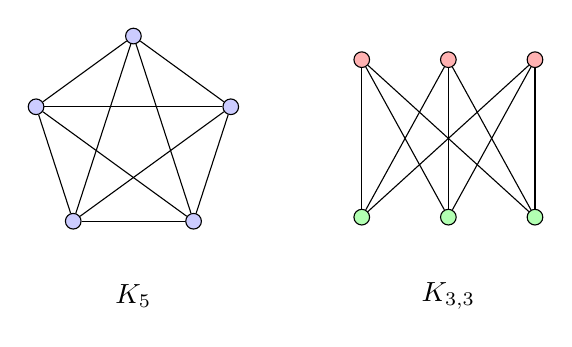
\begin{tikzpicture}[v/.style={circle, draw, fill=blue!20, inner sep=2pt}]
\foreach \i in {0,...,4} \node[v] (a\i) at ({90+72*\i}:1.3) {};
\foreach \i in {0,...,4} \foreach \j in {0,...,4} { \ifnum\i<\j \draw (a\i) -- (a\j); \fi }
\begin{scope}[xshift=4cm]
\foreach \i in {0,1,2} { \node[v, fill=red!30] (u\i) at (\i*1.1-1.1, 1) {}; \node[v, fill=green!30] (w\i) at (\i*1.1-1.1,-1) {}; }
\foreach \i in {0,1,2} \foreach \j in {0,1,2} \draw (u\i) -- (w\j);
\end{scope}
\node at (0,-2) {$K_5$}; \node at (4,-2) {$K_{3,3}$};
\end{tikzpicture}
\end{document}
